\documentclass{standalone}

\usepackage{tikz}
\usepackage{tkz-euclide}
\usepackage{rwthcolors}
\usetikzlibrary{shapes.arrows}
\usetikzlibrary{shapes,decorations,shadows,calc, arrows,arrows.meta}
\usetikzlibrary{decorations.pathmorphing, 
	decorations.markings,decorations.pathreplacing}
\usetikzlibrary{fit,patterns,bending}
\usepgflibrary{arrows}
\usetikzlibrary{trees}
\usetikzlibrary{backgrounds}
\usepackage{fontawesome}


\begin{document}


% !TEX root = ../main.tex

\begin{tikzpicture}

%%%%%%%%%%%%%%%%%%% TOP PART

% INPUT
\node[inner sep=0pt] (input) at (0,0)
{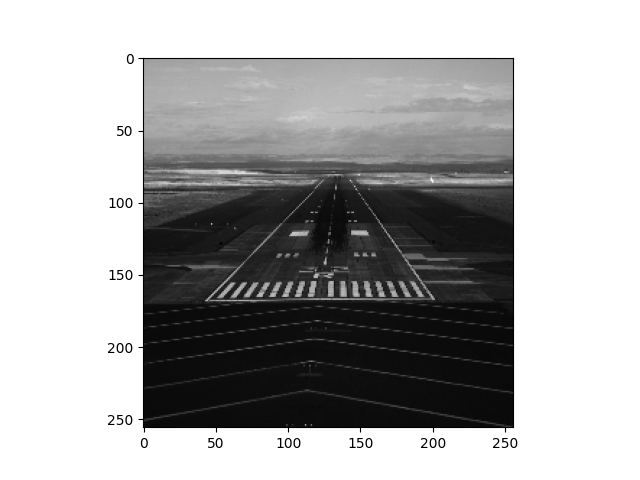
\includegraphics[width=.15\textwidth,trim={3.7cm 2cm 3.5cm 
2cm},clip]{images/input}};
%\node[below of=input, node distance=1.5cm] (input-label) 
%{Input image};

\node[right of=input, node distance=2cm,green50,single arrow, 
fill=green50, 
minimum width = 10pt, single arrow head extend=3pt,
minimum height=5mm] (arrow1) {}; % length of arrow
	
% NETWORK
\node[right of=arrow1,node distance=2cm] (network) 
% {\scalebox{0.8}{\input{imgs/nnet}}};
{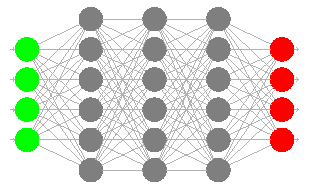
\includegraphics[width=.19\textwidth, clip]{images/neuralagent.pdf}};
%\node[below of=network, node distance=1.5cm] (network-label) 
%{U-Net};

\node[right of=network, node distance=2cm,green50,single arrow, 
fill=green50, 
minimum width = 10pt, single arrow head extend=3pt,
minimum height=5mm] (arrow2) {}; % length of arrow

%OUTPUT
\node[right of=arrow2, node distance=2.5cm] (output) 
{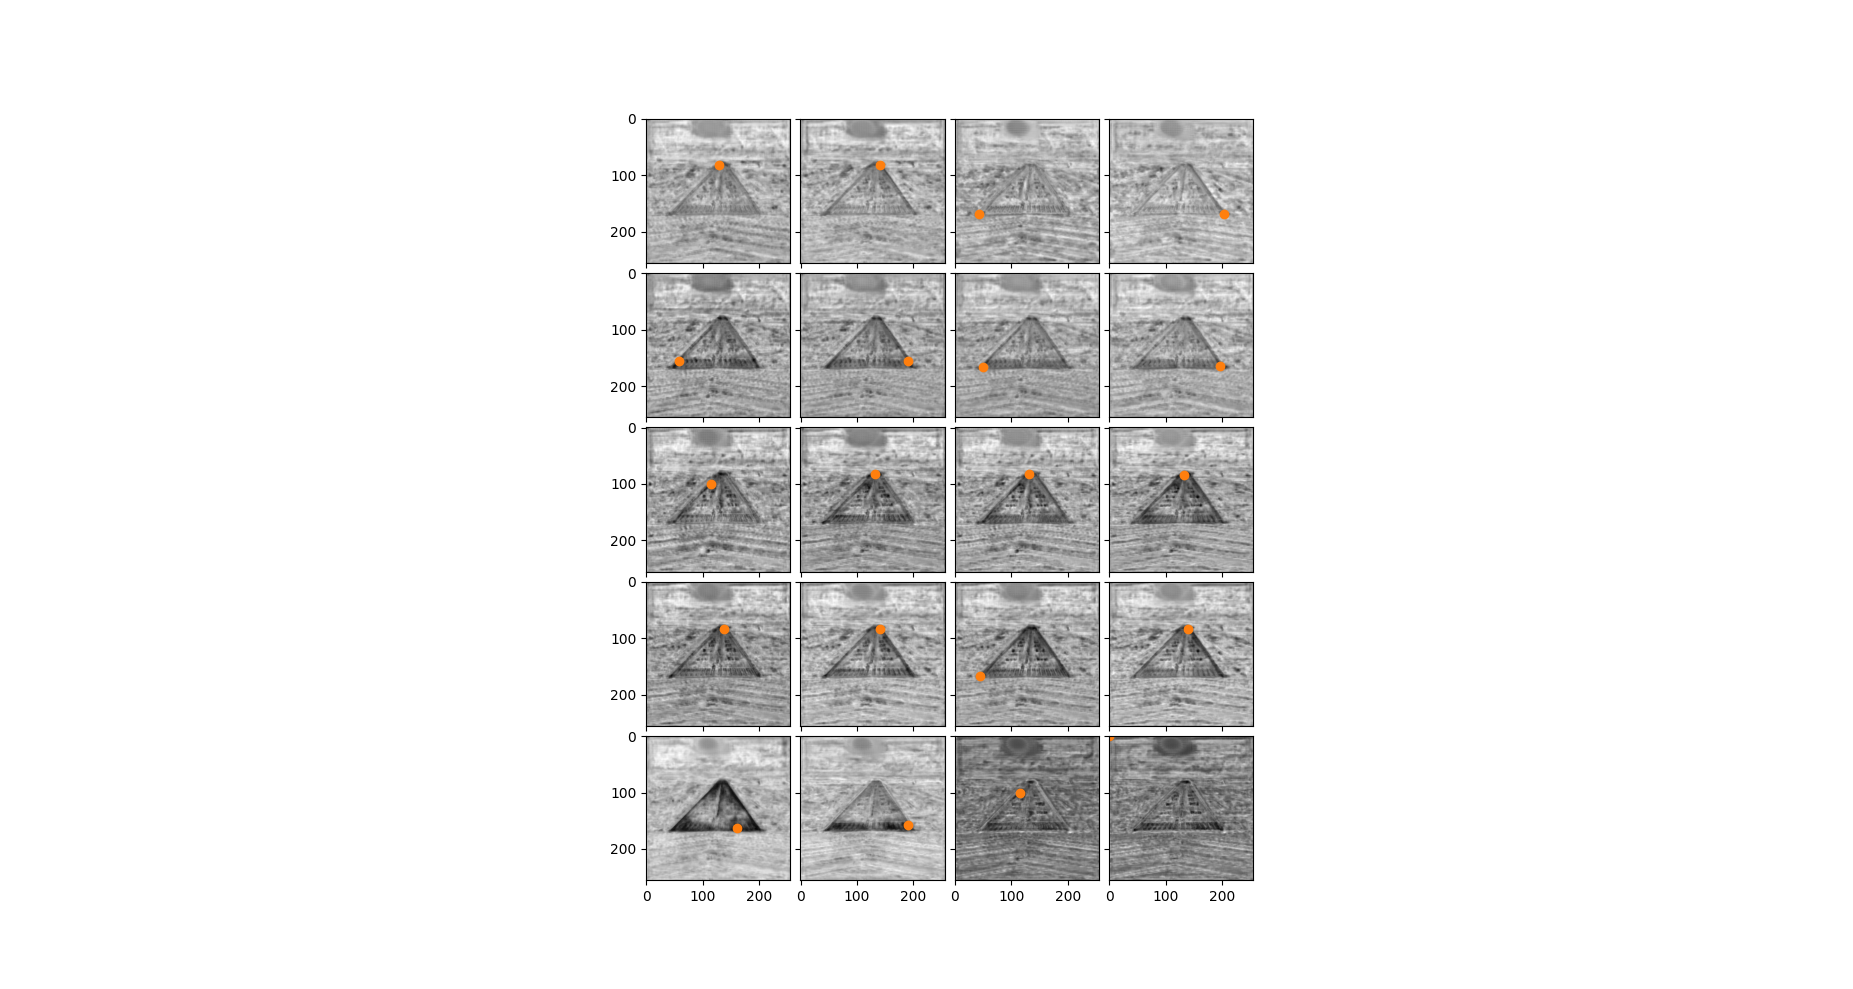
\includegraphics[width=.2\textwidth,trim={16.37cm 6.5cm 15cm 
		1.6cm},clip]{images/output}};
%\node[below of=output, node distance=1.5cm] (output-label) 
%{Segmented output};

\node[thick,draw,rounded corners=3mm,right of=network,node 
distance=2.3cm,black75,minimum width=350pt,minimum height=145pt,xshift=-1.75cm, 
yshift=-0.15cm] 
(segmentation) {};
\node[above of=segmentation, node distance=1.5cm,xshift=-4cm,yshift=0.7cm] 
(segmentation-label) 
{\textbf{Semantic segmentation}};

%%%%%%%%%%%%%%%%%%% BOTTOM PART

\node[right of=network, xshift=4cm, node distance=3.5cm,green50,single arrow, 
fill=green50, 
minimum width = 10pt, single arrow head extend=3pt,
minimum height=5mm,rotate=0,yshift=0cm] (arrow3) {}; % length of arrow

\node[right of=arrow3, node distance=5cm] (pnp_input)
{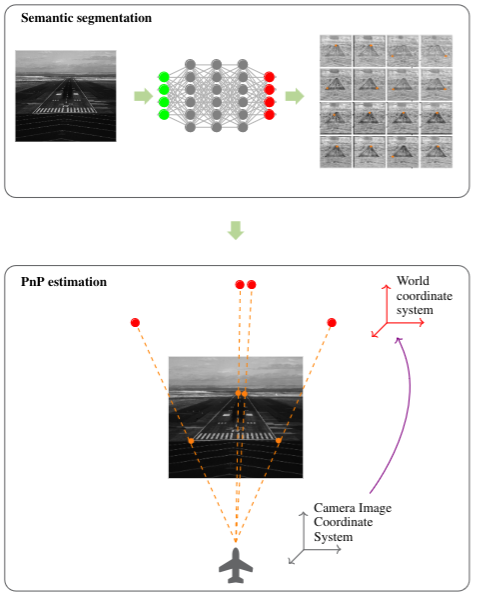
\includegraphics[width=.2\textwidth,trim={3.7cm 2cm 3.5cm 
		2cm},clip]{images/pnp}};
	
\node[below of=pnp_input, node distance=4cm, rotate=45, black75](airplane) 
{\scalebox{3}{\faPlane}};

% plane coordinate system
\draw[thick,->,black75] (6.3,-12,0) -- (7.3,-12,0) node[anchor=north east]{};
\draw[thick,->,black75,align=left] (6.3,-12,0) -- (6.3,-11,0) node[anchor=north 
west]{};
\draw[thick,->,black75] (6.3,-12,0) -- (6.3,-12,1) node[anchor=south]{};
\node[align=left] at (7.6,-11.3) {Camera Image\\ Coordinate\\ System};


% first dot (from left)
\draw [dashed, orange, thick]  (4.5,-11.8) -- (1.85,-6);
\node[mark size=3pt,color=red] at (1.85,-6) {\pgfuseplotmark{*}};

% second dot
\draw [dashed, orange, thick]  (4.5,-11.8) -- (4.62,-5);
\node[mark size=3pt,color=red] at (4.62,-5) {\pgfuseplotmark{*}};

% third dot
\draw [dashed, orange, thick]  (4.5,-11.8) -- (4.93,-5);
\node[mark size=3pt,color=red] at (4.93,-5) {\pgfuseplotmark{*}};

% fourth dot
\draw [dashed, orange, thick]  (4.5,-11.8) -- (7.05,-6); 
\node[mark size=3pt,color=red] at (7.05,-6) {\pgfuseplotmark{*}};

% world coordinate system
\draw[thick,->,red] (8.5,-6,0) -- (9.5,-6,0) node[anchor=north east]{};
\draw[thick,->,red,align=left] (8.5,-6,0) -- (8.5,-5,0) node[anchor=north 
west]{};
\draw[thick,->,red] (8.5,-6,0) -- (8.5,-6,1) node[anchor=south]{};
\node[align=left] at (9.5,-5.3) {World\\ coordinate\\ system};

% transformation
\draw [thick, violet, ->, shorten <= 2.3cm, shorten >= 0.5cm] (6.3,-12,0) 
to[out=40,in=-50] (8.5,-6,0);

\node[thick,draw,rounded corners=3mm,right of=network,node 
distance=2.3cm,black75,minimum width=350pt,minimum height=245pt,xshift=-1.75cm, 
yshift=-8.8cm] 
(pnp) {};
\node[above of=pnp, node distance=1.5cm,xshift=-4.6cm,yshift=2.4cm] 
(pnp-label) 
{\textbf{PnP estimation}};





 
%\node[below of=arrow2,red50] (repeat) 
%{\rotatebox{-180}{\scalebox{3}{\faRepeat}}};


		
\end{tikzpicture}
		

\end{document}
